% this TeX file provides an awesome example of how TeX will make super 
% awesome tables, at the cost of your of what happens when you try to make a
% table that is very complicated.
% Originally turned in for Dr. Nico's Security Class
\documentclass[11pt]{article}


% Use wide margins, but not quite so wide as fullpage.sty
\marginparwidth 0.5in 
\oddsidemargin 0.25in 
\evensidemargin 0.25in 
\marginparsep 0.25in
\topmargin 0.25in 
\textwidth 6in \textheight 8 in
% That's about enough definitions

% multirow allows you to combine rows in columns
\usepackage{multirow}
% tabularx allows manual tweaking of column width
\usepackage{tabularx}
% longtable does better format for tables that span pages
\usepackage{longtable}
\usepackage[T1]{fontenc}
\usepackage[polish]{babel}
\usepackage[utf8]{inputenc}
\usepackage{graphicx}

\begin{document}
% this is an alternate method of creating a title
%\hfill\vbox{\hbox{Gius, Mark}
%       \hbox{Cpe 456, Section 01}  
%       \hbox{Lab 1}    
%       \hbox{\today}}\par
%
%\bigskip
%\centerline{\Large\bf Lab 1: Security Audit}\par
%\bigskip
\author{Szymon Bagiński}
\title{\textbf{\centerline{Bezpieczeństwo usług sieciowych}} \newline Laboratorium 1: Komunikator z szyfrowaniem}
\maketitle

\section{Cel zadania}

Celem zadania było przygotowanie komunikatora (czatu) klient-serwer wspierającego bezpieczną wymianę sekretu (przy użyciu protokołu Diffiego-Hellmana). Komunikator musiał wspierać szyfrowanie wiadomości zgodnie z następującym formatem danych opartym o JSON:

\begin{center}
    \begin{tabular}{ | l | c | r |}
      \hline
      Stage & A (client) & B (server) \\ \hline
      1 & \{ “request”: “keys” \} -> & \\ \hline
      2 &  & <- \{ “p”: 123, “g”: 123 \} \\ \hline
      3 & \{ “a”: 123 \} -> & <- \{ “b”: 123 \} \\ \hline
      4 & \{ “encryption”: “none” \} -> &  \\ \hline
      5 & \{ “msg”: “...”, “from”: “John” \} -> & <- \{ “msg”: “...”, “from”: “Anna” \} \\
      \hline
    \end{tabular}
\end{center}

\begin{enumerate}
    \item Po połączeniu do serwera klient prosi o liczby p oraz g.
    \item Serwer wysyła do klienta liczby p oraz g.
    \item Serwer i klient wymieniają się publicznymi wartościami A oraz B:
        \begin{enumerate}
            \item Klient wysyła do serwera obliczoną wartość A.
            \item Serwer wysyła do klient obliczoną wartość B.
        \end{enumerate}
        Kroki a oraz b mogą nastąpić w dowolnej kolejności.
    \item *OPCJONALNIE* Klient wysyła do serwera informację o żądanym sposobie szyfrowania wiadomości. Jeżeli klient nie wyśle tej informacji, to strony przyjmują domyślne szyfrowanie ustawione na “none”.
    \item Klient oraz serwer wymieniają się szyfrowanymi wiadomościami.
\end{enumerate}

Treść wiadomości powinna być zakodowana za pomocą base64 przed umieszczeniem jej w strukturze JSON.
\newpage
Wspierane metody szyfrowania:
\begin{itemize}
    \item none - brak szyfrowania (domyślne)
    \item xor - szyfrowanie xor jedno-bajtowe (należy użyć najmłodszego bajtu sekretu)
    \item cezar - szyfr cezara
\end{itemize}


\section{Wykonanie zadania}

\subsection{Technologia}

Do wykonania zadania postanowiono skorzystać z języka programowania \textbf{Rust}. Jest to stosunkowo nowy język ukierunkowany na bezpieczeństwo oraz wysoką wydajność tworzonych programów. Zadanie potraktowano jako pewnego rodzaju eksperyment z tym językiem, żeby się z nim zapoznać.

Aby działać poprawnie, komunikator musi wysyłać i odbierać dane przez gniazda sieciowe.
Może się wydawać, że jest to proste zadanie, ale istnieje kilka sposobów o różnej złożoności, efektywnej obsługi operacji wejścia i wyjścia. Główna różnica między podejściami polega na traktowaniu blokowania: domyślnie zapobiega się wszelkim operacjom CPU, podczas gdy czekamy, aż dane dotrą do gniazda sieciowego. Ponieważ nie możemy pozwolić jednemu użytkownikowi naszej usługi czatu blokować innych, musimy jakoś je wyizolować.

Najczęstszym sposobem jest utworzenie oddzielnego wątku dla każdego użytkownika, tak aby blokowanie zadziałało tylko w kontekście pojedynczego wątku. Ale chociaż koncepcja jest prosta i taki kod jest łatwy do napisania, każdy wątek wymaga pamięci dla swojego stosu i ma narzut przełączników kontekstu - nowoczesne procesory serwera mają zwykle około 8 lub 16 rdzeni, a pojawianie się wielu wątków wymaga od jądra systemu operacyjnego ciężkiej pracy, aby przełączać między nimi wykonanie z odpowiednią prędkością. Z tego powodu trudno jest skalować wielowątkowość do wielu połączeń.

Zamiast tego użyjemy wydajnych interfejsów systemu, które wykorzystują pętlę zdarzeń (event loop). Działają one w prosty sposób: bajty przychodzą przez sieć, docierają do gniazd, a zamiast czekać, kiedy dane staną się dostępne dla odczytu, mówimy gniazdu, aby nas powiadomić o nadejściu nowych danych.

Powiadomienia przychodzą w formie zdarzeń, które są obsługiwane przez pętle zdarzeń [Rysunek \ref{fig:model}]. I tu właśnie dzieje się blokowanie: zamiast okresowych kontroli tysięcy gniazd, czekamy tylko na pojawienie się nowych zdarzeń. To ważne różnica, ponieważ szczególnie w aplikacjach sieciowych bardzo często zdarza się, że wielu bezczynnych klientów czeka na jakąś aktywność. Dzięki asynchronicznym operacjom wejścia / wyjścia będziemy mieli bardzo niewiele narzutów na uchwytach gniazda.

Aby zaimplementować opisane podejście skorzystano z biblioteki mio (Metal IO), która kładzie nacisk na jak najmniejsze obciążenie. Dzięki niej powstała maszyna stanów obsługująca każde połączenie z klientem.

\begin{figure}
    \centering
    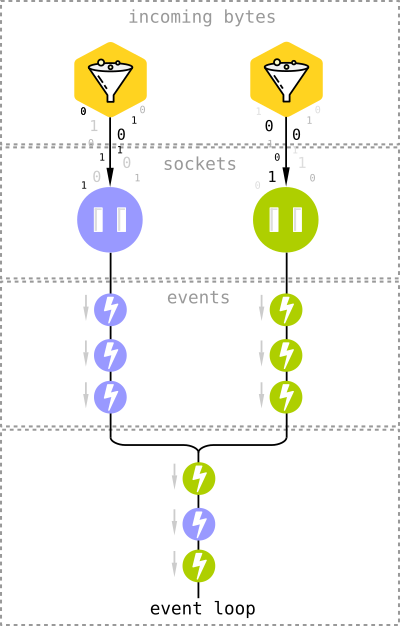
\includegraphics[width=0.35\textwidth]{io-multiplex.png}
    \caption{Schemat modelu opartego o zdarzenia}
    \label{fig:model}
\end{figure}

\subsection{Generowanie parametrów protokołu Diffiego-Hellmana}

W programie server zaimplementowano dynamiczne generowanie parametrów wysyłanych do każdego klienta, na podstawie których potem oblicza się numery publiczne oraz sekret. 

W pod module serwera \texttt{parameters.rs} znajduje się funkcja \texttt{generate\_parameters}, która tworzy nowy zestaw parametrów. W tym celu najpierw wybierana jest losowa liczba pierwsza \textit{p}. W tym przypadku jest to liczba pierwsza z zakresu <9001, 10007>. Drugi parametr \textit{g} jest wybierany losowo spośród wszystkich pierwiastków pierwotnych modulo \textit{p}. Z uwagi na fakt, że znajdowanie pierwiastków pierwotnych jest stosunkowo czasochłonną operacją zdecydowano się na niewielkie liczby. Implementacja rozwiązania pozwala jednak na szybką zmianę możliwych wartości parametrów. 

\subsection{Ważne funkcjonalności systemu}

\begin{itemize}
    \item Serwer wspiera wielu klientów
    \item Kolejność wymiany wartości A i B jest dowolna
    \item Parametry protokołu Diffiego-Hellmana są generowane dynamicznie
    \item Parametry protokołu Diffiego-Hellmana są różne dla każdego klienta
    \item Z punktu widzenia serwera wiadomość o szyfrowaniu jest opcjonalna, natomiast klient zawsze ją wysyła nawet gdy nie jest ona ustawiona
    \item Serwer, w trakcie połączenia z klientem, zmieni sposób szyfrowania jeśli otrzyma odpowiednie żądanie. Jednak program klienta nie udostępnia sposobu wysłania ponownego żądania ustawienia szyfrowania. 
\end{itemize}

\subsection{Korzystanie}

Aby korzystać z komunikatora należy najpierw uruchomić program \textbf{server}, a następnie dowolną ilość programów \textbf{client}, które posiadają tylko interfejs konsolowy (sposób uruchomienia został opisany w pliku README). Każda wpisana linia jest interpretowana jako nowa wiadomość i rozsyłana do pozostałych użytkowników. Równolegle są pokazywane wiadomości od innych użytkowników połączonych z tym samym serwerem. Wiadomości te nie są jednak przechowywane na serwerze, więc klient podłączony po przyjściu danego komunikatu nie będzie w stanie go otrzymać.

\section{Podsumowanie}

Wykonanie zadania zajęło dużo więcej czasu niż założono na początku. Spowodowane było to przede wszystkim nieznajomością technologii oraz wyborem bibliotek. Nie mają one w znacznej większości stabilnej wersji, a ich interfejs się znacząca różni między wersjami. Jest to zrozumiałe, ponieważ otoczenie języka \textbf{Rust} jest relatywnie młode i się dynamicznie rozwija. Materiały edukacyjne i różnego rodzaju tutoriale nie są w sieci mocno rozpowszechnione w porównaniu do innych technologii, a dokumentacja często pozostawia wiele do życzenia.

Niemniej jednak założenia zadania udało się wypełnić w zdecydowanej większości, przy okazji zdobywając nową wiedzę i doświadczenia z \textbf{Rust}-em. Specyficzna składnia tego języka oraz pewien rygor programowania w nim pozwala uniknąć wielu błędów podczas programowania, co w przypadku komunikacji sieciowej jest istotne. Język ten staje się także po pewnym czasie, gdy zrozumie się podstawowe koncepty takie jak zarządzanie pamięcią, wygodny i intuicyjny.

\end{document}
